\chapter{Pre Study}
During the exploratory phase, we aimed to limit the scope of this study to only cover merge-conflicts related to a specific branching strategy. We studied the possibilities for limit the scope to feature-branching-related merge-conflicts or to variance-related merge-conflicts.
\section{Feature-Branching}
To detect feature branches, we proposed some indicators. The commit messages and the branch names may contain clues. A commit message could contain the branch name, however, since commit messages might be edited by the committee, it is unreliable to find feature branches this way.
\paragraph*{}
In the git history, branch names might indicate if it is a feature branch, however due to how Git handles branches it proved to be difficult. When two branches are to be merged, there are two different options: merge or rebase. When merging, git takes the two commits that are to be merged and creates a new commit which, unlike other commits, has two ancestral commits, being the two commits that were merged. This makes it possible to distinguish merge commits from other forks and thus makes it possible to analyze them separately. Sometimes, rebase is used instead of merging. This means that instead of creating a merge commit, an ordinary commit is created. That commit consists of a snapshot, in which the changes introduced in the branch that is to be merged in, are applied on top of the commit that the branch which was rebased into points at. Then, both branches that were to be rebased are then changed to point at the new commit, which has only one parent, being the commit that the branch which was to be rebased into was pointing at. The other commit is left as it was. Thus, there is no straight-forward way of find those rebased commits.
\paragraph*{}
To be able to understand what happened historically in a git-hosted project, one must have a basic knowledge about how Git works. To analyze historical branches and merges is more difficult than one might expect. A question that one might ask is “In what branch was this commit made?”. A Git branch is only a reference that points to the latest commit, and does not “contain” commits. There is also a reference called HEAD, which points to the currently checked out branch. When a branch is merged, the branch will point at the same commit as the branch it was merged into. Therefore, a more correct way to ask this is “At what branch did HEAD point during the creation of this commit?”. That information is not stored in Git and therefore, that question is not possible to answer. There is no information that tells which branch was merged into which. However, clues may be found in commit messages but, as they are often edited, they are not reliable.
\begin{figure}
    \centering
    \begin{subfigure}[b]{0.3\textwidth}
        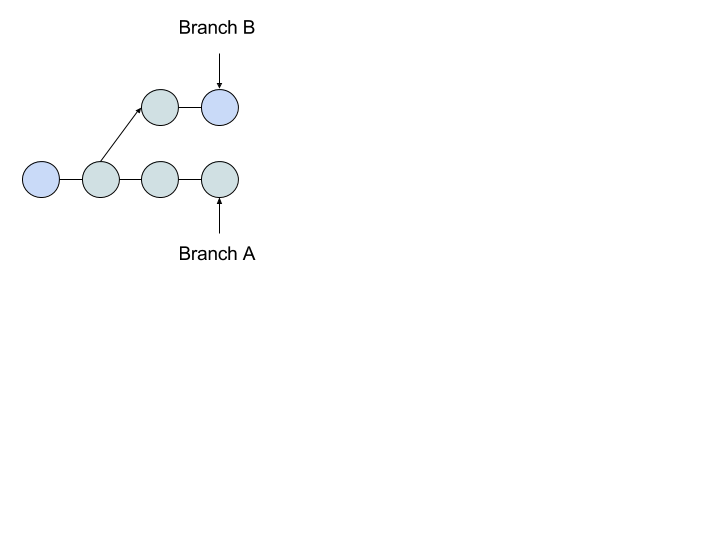
\includegraphics[width=200pt]{figure/branch1.png}
        \caption{The branches Branch A and Branch B both points at their respective tip commit.}
        \label{fig:branch1}
    \end{subfigure}
    ~ %add desired spacing between images, e. g. ~, \quad, \qquad, \hfill etc. 
      %(or a blank line to force the subfigure onto a new line)
    \begin{subfigure}[b]{0.3\textwidth}
        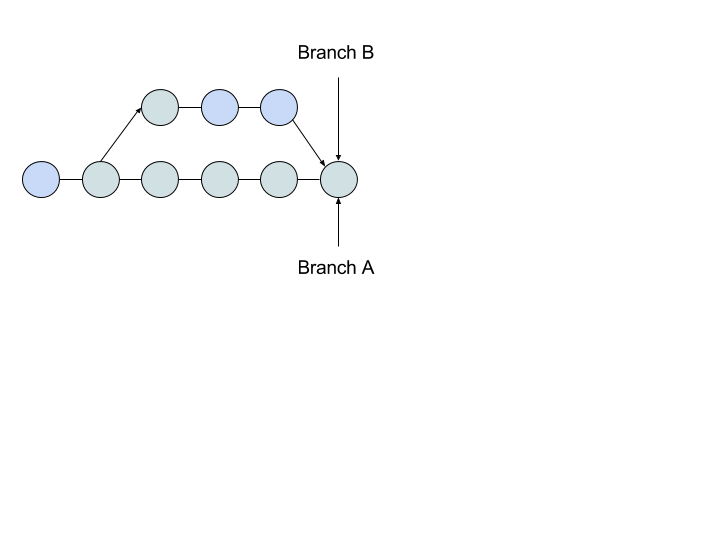
\includegraphics[width=200pt]{figure/branch2.png}
        \caption{When merged, both branches points at the merge commit.}
        \label{fig:branch2}
    \end{subfigure}
    ~ %add desired spacing between images, e. g. ~, \quad, \qquad, \hfill etc. 
    %(or a blank line to force the subfigure onto a new line)
    \begin{subfigure}[b]{0.3\textwidth}
        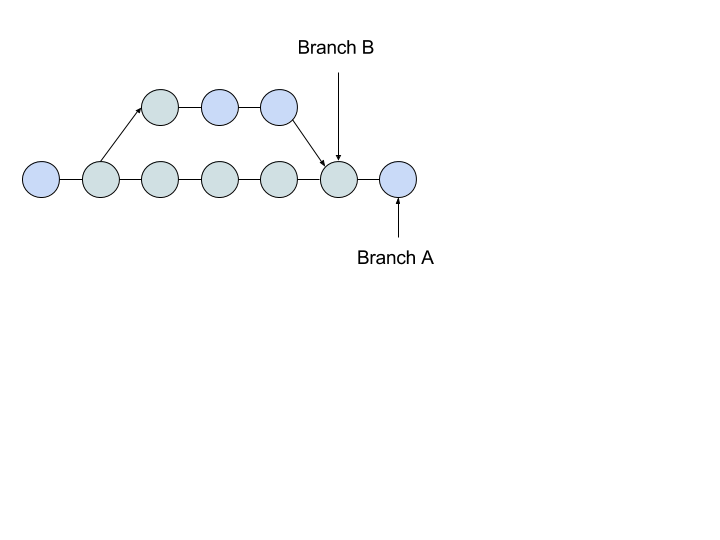
\includegraphics[width=200pt]{figure/branch3.png}
        \caption{If Branch A is checked out and then committed to, Branch B will still point at the merge commit.}
        \label{fig:branch3}
    \end{subfigure}
    \caption{Branches}\label{fig:branches}
\end{figure}
\paragraph*{}
Moreover, using the command
\lstset{language=Bash}
\begin{lstlisting}[frame=single]
git branch --contains <SHA-1>
\end{lstlisting}
will show the “branches whose tip commits are descendants of the named commit”¹. Therefore it is impossible to know, using this information alone, which branch was merged into which and also which branch a commit was created on. Common practice amongst developers is to delete a branch after it has been merged, and once that happens, all information about that branch is lost from the Git history.
\section{Variance-Branching}
To detect variance-related branches, we proposed the following indicators: Pull-requests, introduced boolean parameters, name of introduced boolean parameters, time in a branch’s lifetime that the parameters were introduced, the existence of clones. In variance-related merge-conflicts, we wanted to study how variants in code emerge in different branches.
\subsection{Repositories to analyze}
We want to analyse fairly big projects that contain many commits and many forks along with many branches. This is because we want to cover as much of variant possibilities as possible to identify interesting and widespread conflict resolution patterns. To satisfy these requirements, the 20 top starred Java repositories on GitHub were chosen.
\paragraph*{}
The projects listed in Table (no) were cloned so that Git commands could be used to analyze the repositories. Elasticsearch was chosen as the project for our initial analysis since it has a vast number of commits (more than 20000) and forks.
\paragraph*{}
Elasticsearch is a distributed search engine used for analysing data in realtime.  %FOOT NOTE
\paragraph*{}
(As of 23/3-16)\\
\begin{tabular}{ l l l l}
\hline
\multicolumn{1}{c}{\textbf{Name}} & \multicolumn{1}{c}{\textbf{Commits}} & \multicolumn{1}{c}{\textbf{Branches}} & \multicolumn{1}{c}{\textbf{Forks}}\\
Elasticsearch & 20712 & 46 & 5229\\
Android-async-http & 856 & 3 & 4024\\
Android-best-practices & 201 & 1 & 1696\\
Android-universal-image-loader & 1025 & 3 & 5640\\
Curator & 1050 & 9 & 304\\
Eventbus & 404 & 5 & 2493\\
Fresco & 494 & 3 & 2453\\
Guava & 3372 & 4 & 1862\\
Iosched & 129 & 2 & 4071\\
Java-design-patterns & 1196 & 6 & 3495\\
Leakcanary & 238 & 15 & 1291\\
Libgdx & 12247 & 4 & 4479\\
Okhttp & 2449 & 37 & 2518\\
React-native & 5707 & 23 & 5609\\
Retrofit & 1285 & 21 & 2081\\
Rxjava & 4630 & 24 & 1919\\
Slidingmenu & 336 & 8 & 5306\\
Spring-framework & 11825 & 10 & 6860\\
Storm & 1764 & 44 & 1760\\
Zxing & 3203 & 3 & 4730
\end{tabular}
\subsection{Data Gathering Tool}
When studying the code of Elasticsearch, we noticed that parameters were introduced and loaded from an external configuration file. These parameters were then used to set boolean variables that usually indicate whether to use a certain block of code or not. In Elasticsearch, the function used to set these boolean variables was called “getAsBoolean” and takes a string parameter name, and a boolean default value.\\
\lstset{language=Java}
\begin{lstlisting}[frame=single]
boolean example = getAsBoolean("example_parameter", true);
\end{lstlisting}
\paragraph*{}
The "example\_parameter" could be set by the user in the external configuration file and if it has not been set, a default value, in this example true, will be used. The boolean variable would in some cases be used to indicate which block of code to use, as in this example taken from a snippet of Elasticsearch code:\\
\lstset{language=Java}
\begin{lstlisting}[frame=single]
this.autoThrottle = indexSettings.getAsBoolean(AUTO_THROTTLE, true);

if (autoThrottle) {
   concurrentMergeScheduler.enableAutoIOThrottle();
} else {
   concurrentMergeScheduler.disableAutoIOThrottle();
}
\end{lstlisting}
\paragraph*{}
To be able to identify the parameters, and collect data about them, a tool was developed in Java which would gather the data automatically. All data that is stored in Git is hashed using SHA-1. If not stated otherwise, in this document, the hash will be referred to by SHA-1. The data to be gathered includes:
\begin{itemize}
\item The parameter name that was introduced
\item The commit SHA
\item The if-statement that the boolean is used in
\item The code where the boolean variable is set by the function that takes the parameter name as one of its parameters.
\item The commit message
\item Whether or not the commit was a pull request \ldots
\end{itemize}
The data was gathered by developing a Java program which uses Linux bash scripts that executes Git commands to get the desired data. As Git saves the data as snapshots and not as changes, one needs to compare two commits in order to see which changes that were introduced in a commit. To do this, we use the built in diff command in the following way: % FOOT NOTE
\lstset{language=Bash}
\begin{lstlisting}[frame=single]
git --no-pager diff <SHA-1>^ <SHA-1>
\end{lstlisting}
where \^ is a git shortcut to get the parent commit of a commit SHA-1.
\paragraph*{}
\textbf{Parameter name.} The parameter name was extracted from the line where the boolean is set by the getAsBoolean function. It is useful to include it in the data so that it can be used when manually looking through the code to understand what the parameter was used for.
\paragraph*{}
\textbf{Commit SHA-1.} For every commit that is checked out, we search for parameters and if there exist at least one, the commit SHA-1 is saved so that we know which commits to check out when we want to look manually at the code.
\paragraph*{}
\textbf{If-statement the boolean is used in.} In the beginning of developing the tool, we extracted the newly introduced boolean variables that was later used in if-statements. This proved to be not useful since the boolean variable names was not always the same as the parameter names used in the configuration file.
\paragraph*{}
\textbf{getAsBoolean line.} While extracting the name of the parameter in the getAsBoolean function, we also save the line itself to be able to quickly see the name of the boolean variable as well as the default value the boolean will be assigned to if the parameter is not set. This data is printed to the excel document.
\paragraph*{}
\textbf{Commit message.} The commit message is also extracted and printed in the excel document. In case the commit message contains important information which could indicate that the commit contains variant related code, it is vital to look at it to find which commits are good to analyse manually.
To get the commit message for a giver SHA-1, this command was used:
\lstset{language=Bash}
\begin{lstlisting}[frame=single]
git log --format=%B -n 1 <SHA-1>
\end{lstlisting}
\paragraph*{}
\textbf{Pull request.}When changes on a branch in a fork of a project is to be merged into the original project, pull-requests are used. It is interesting to know whether or not the commit was a pull request. Finding out if variant related code is more or less likely in pull requests would be interesting for the study. To know whether a given merge commit was a pull request, the commit message was parsed to see if it contains "Merge pull request \#".
\subsection{Find Details about Introduced Parameter}
Branches consist of one or more commits and often when new functionality is added or changed to software, good practice is to branch out, therefore developers tend to do just that. When new parameters are added that decides which variant of code to use, we believe this most often happens in a new branch, and it will be interesting for the study to know at which point in life of the branch this happens.
\paragraph*{}
To analyse when in the branch a parameter was introduced, we extended our tool to calculate when a given parameter was introduced in a branch, given the merge commit where the branch was merged back into the original branch and the parameter name. By recursively step backwards from the merge commit, through the commits of the branch, searching for the given parameter, finding the commit where it was introduced would be straight-forward, we thought. Due to limitations in the Git history regarding branches, we soon found out that analysing commits with regards to branches is very limited, if not impossible in some cases.
\paragraph*{}
Another question one might ask is “How many branches does this project have?”. That can be answered using the git command:
\lstset{language=Bash}
\begin{lstlisting}[frame=single]
git branch -a
\end{lstlisting}
However, as it is common practice to delete branches after they have been merged, the command is of little use as it only lists the currently existing branches. Information about old branches may be found in commit messages but, again, as they are often edited, they are not reliable.
\paragraph*{}
In yet another attempt to find variant-related merges, we sought to find merge-commits where a new parameter was introduced to solve conflicts. In Elasticsearch, the parameters we looked for was fetched using “getAsBoolean”. It turned out that there was not a single example of such a case where “getAsBoolean” was introduced in a merge-commit in the history of Elasticsearch.
\section{Outcome of the Pre Study}
The pre study has shown that it is difficult to detect whether merge-commits are related to variance or feature-branches. Thus we decided that the direction of this study will be to identify and classify merge-conflict resolution patterns in general. The list of conflict patterns by Accioly will be used to map the conflicting pattern to it’s corresponding resolution patterns.
\paragraph*{}
The tool created during the prestudy will be used when analyzing merge-conflict resolution patterns. It will be used to parse information about commits in GitHub repositories and also be extended with new functionality to automatically be able to identify the resolution patterns.